\documentclass[a4]{article}
\usepackage[english]{babel}
\usepackage{fullpage}
\usepackage{fancyhdr}
\usepackage{amsmath,amsfonts,amsthm,amssymb}

\usepackage{../shortcuts_fb}
\usepackage{csquotes}
\usepackage[titlenumbered,ruled,noend,french,onelanguage]{algorithm2e}
\usepackage{hyperref}
\usepackage{cleveref}
\usepackage[titlenumbered,ruled,noend]{algorithm2e}
\usepackage{multirow}
\usepackage{subcaption}
\usepackage[super]{nth}
\pagestyle{fancy}
\lhead{Creation : 09/02/2021}
\chead{PGD}
\rhead{}

\SetKwFor{FOR}{For}{do}{end For}%

\usepackage[round]{natbib}
\bibliographystyle{plainnat}

\setlength{\headsep}{13.6pt}
\headheight=14.85pt
%\renewcommand{\chaptermark}[1]{\markboth{\thechapter.\ #1}{}}
\renewcommand{\sectionmark}[1]{\markright{\thesection\ #1}}

\renewcommand{\headrulewidth}{0.5pt}
\addtolength{\headheight}{0.5pt}
\renewcommand{\footrulewidth}{0.pt}
\fancypagestyle{plain}{\fancyhead{} \renewcommand{\headrulewidth}{0pt}}

\title{ElasticNet minimization with interactions and gradient descent based solvers with GPU}
\author{
  Lefort, Tanguy\\
  \texttt{tanguy.lefort@etu.umontpellier.fr}
  \and
  Bascou, Florent\\
  \texttt{florent.bascou@umontpellier.fr}
  \and
  Lèbre, Sophie\\
  \texttt{sophie.lebre@umontpellier.fr}
  \and
  Charlier, Benjamin\\
  \texttt{benjamin.charlier@umontpellier.fr}
  \and
  Salmon, Joseph\\
  \texttt{joseph.salmon@umontpellier.fr}
}

\begin{document}

\maketitle

%%%%%%%%%%%%%%%%%%%%%%%%%%%%%%%%%%%%%%%
%% Introduction
%%%%%%%%%%%%%%%%%%%%%%%%%%%%%%%%%%%%%%%

\section*{Introduction}

Penalized linear models are now frequent when working with large datasets. Especially when the number of features is quite large,
we need to perform some kind of feature selection to keep the benefits of the interpretability.
Methods such as LASSO \citep{Tibshirani96} or ElasticNet \citep{Zou_Hastie05} use a combination of $\ell_1$ and $\ell_2$ penalties to take into account the sparsity but also the correlation amongst the features.

\medskip

If we add in the linear model the first order interactions, the matrix stored quickly become very large (in the order of the number of features squared) and
solvers can be very time consuming. For these reasons, using methods that exploit the architecture of the problem may be useful.
In particular, recent developements using GPU acceleration can help to accelerate such solvers, at the cost of using reasonable-sized matrices.
Here we compare a coordinate descent \citep{Bascou_Lebre_Salmon20} with proximal gradient descent algorithms \citep{Beck17}.
We exploit the structure by block of the interaction matrix to use the cyclic block proximal gradient method.
We also look at the interaction matrix with all the interactions including redundant ones and write the equivalence between our problems with the corresponding proximal operators.

%%%%%%%%%%%%%%%%%%%%%%%%%%%%%%%%%%%%%%%
%% Notation
%%%%%%%%%%%%%%%%%%%%%%%%%%%%%%%%%%%%%%%

\section*{Notations}

\paragraph{General notations.}
We denote $[k]=\{1, \dots, k\}$. For any matrix $A$, $A_{ij}$ is its $(i,j)$-entry, $a_j$ the $j$-th column
and $a_i$ the $i$-th row. For a subset $\mathcal{J} \subset [k]$, $A_{\mathcal{J}}$ is the sub-matrix $(a_j)_{j\in \mathcal{J}}$ with $|\mathcal{J}|$ columns.
We use the same notation on a vector to consider the components of those indexes.
The $2$-norm $\norm{A}_2$ is the largest singular value of $A$. Finally, for two vectors $u,v\in\bbR^k$, $(u\odot v)_i=u_iv_i$ is the element-wise product.

\paragraph{For our data.}
In the followings, we will consider our dataset the matrix $X=[x_1,\dots, x_p]\in\bbR^{n\times p}$.
We use $\tau_K : [p]^2 \longrightarrow [K]$ a function to index our interactions. Meaning that for the interaction matrix $Z$, $Z_{\tau_K(i,j)} = x_i\odot x_j$.
If we exclude redundant interactions, then $K=q=p(p+1)/2$, else $K=\widetilde q=p^2$. In the later case, we write $\widetilde Z$ the interaction matrix.
And finally, we define the index of the block generated by $x_j$ as the branch $\branch{K}{j}:=\{\tau_K(j,l),\ l\in [p]\}$.
So for example $Z_{\branch{q}{2}}=[x_2\odot x_2, \dots, x_2\odot x_p]$.


%%%%%%%%%%%%%%%%%%%%%%%%%%%%%%%%%%%%%%%
%% Explain the model and PGD procedure
%%%%%%%%%%%%%%%%%%%%%%%%%%%%%%%%%%%%%%%

\section*{Elastic Net model with interactions}

For a dataset $X\in\bbR^{n\times p}$, the estimator with first order interactions $Z$ reads:
\begin{align} \label{pb:init}
	(\cP) \quad \widehat{p}
	 & = \min_{\substack{\beta \in \bbR^p \\ \Theta \in \bbR^q}}
	\frac{1}{2 n} \norm{y - X\beta - Z\Theta}^2_2 +
	\lambda_{\beta, \ell_1} \norm{\beta}_1 + \lambda_{\Theta, \ell_1} \norm{\Theta}_1 +
	\frac{\lambda_{\beta, \ell_2}}{2} \norm{\beta}_2^2 + \frac{\lambda_{\Theta, \ell_2}}{2} \norm{\Theta}_2^2 \\
	 & = \min_{\substack{\beta \in \bbR^p \\ \Theta \in \bbR^q}}
	f(\beta, \Theta) + g^{(1)}_{\lambda_{\beta, \ell_1}, \lambda_{\beta, \ell_2}}(\beta) + g^{(2)}_{\lambda_{\Theta, \ell_1}, \lambda_{\Theta, \ell_2}}(\Theta)\enspace .
\end{align}

Splitting the two penalty functions allows us to consider a block coordinate descent algorithm for the minimization, alternating the optimization on $\beta$ and on $\Theta$.
Using proximal gradient descent, we obtain the following iterates for the $k-{th}$ step

\begin{align}
	\beta^{k+1}  & =
	\prox_{\frac{1}{L_X}g^{(1)}}
	\left(\beta^k - \frac{1}{L_X}\frac{\partial}{\partial \beta}f(\beta^k, \Theta^k)\right)\enspace, \\
	\Theta^{k+1} & =
	\prox_{\frac{1}{L_Z}g^{(2)}}
	\left(\Theta^k - \frac{1}{L_Z}\frac{\partial}{\partial \Theta}f(\beta^{k+1}, \Theta^k)\right)\enspace,
\end{align}

where $L_X$ and $L_Z$ are Lipschitz constants for the partial derivatives to be determined.
We still need to calculate the derivates of $f$ \wrt each component. Direct computation shows that:

\begin{align}
	\nabla_{\beta}f(\beta, \Theta) = \frac{1}{n}X^\top (X\beta + Z\Theta - y)
	\quad \text{and} \quad
	\nabla_{\Theta}f(\beta, \Theta) = \frac{1}{n}Z^\top (X\beta + Z\Theta -y)\enspace.
\end{align}

Now we can compute the Lipschitz constants. For $\beta$, we have

\begin{align*}
\norm{\frac{\partial}{\partial \beta}f(\beta_1, \Theta) - \frac{\partial}{\partial \beta}f(\beta_2, \Theta)}_2
												& = \frac{1}{n} \norm{ X^\top(X\beta_1 + Z\Theta - y) - X^\top(X\beta_2 + Z\Theta - y) }_2 \\
												& = \frac{1}{n} \norm{ X^\top X\beta_1 - X^\top X\beta_2 }_2 \\
												& \leq \frac{1}{n} \norm{ X^\top X }_2 \norm{ \beta_1-\beta_2 }_2  \enspace.
\end{align*}

We thus obtain that $L_X = \frac{\norm{ X^\top X }_2}{n}$ and with the same method $L_Z = \frac{\norm{ Z^\top Z }_2}{n}$.

%%%%%%%%%%%%%%%%%%%%%%%%%%%%%%%%%%%%%%%
%% Formulae for the prox operator
%%%%%%%%%%%%%%%%%%%%%%%%%%%%%%%%%%%%%%%

\paragraph{Calculating the proximal operator.}

For a function $h(x)=\|x\|_1 + \frac{\gamma}{2}\|x\|_2^2$, we know \citep[p.~189]{Parikh14} that

\[
\prox_{\mu h}(x) = \dfrac{1}{1 + \mu\gamma}\prox_{\mu \|\cdot\|_1}(x) = \dfrac{\sign(x)}{1 + \mu\gamma}(|x| - \mu)_+\enspace.
\]

Let us consider $g^{(1)}$ (as the second function is identical), then:

\begin{align}\label{par:proxi}
	\prox_{\mu g^{(1)}}(\beta) & = \prox_{\mu\lambda_{\beta, \ell_1}{h^{(1)}}}(\beta)                                              \\
	                               & = \dfrac{\sign(\beta)}{1 + \mu \lambda_{\beta,\ell_2}}(|\beta| - \mu\lambda_{\beta, \ell_1})_+\enspace,
\end{align}

with ${h^{(1)}}(\beta) = \|\beta\|_1 + \frac{\lambda_{\beta, \ell_2} / \lambda_{\beta, \ell_1}}{2} \|\beta\|_2^2$
such that $ \lambda_{\beta, \ell_1}{h^{(1)}}(\beta) = g^{(1)}(\beta)$. For the update on $\Theta$, considering $u = \Theta^k - \frac{n}{\norm{ Z^\top Z}} \frac{1}{n} Z^\top (X\beta^{k+1} + Z\Theta^k - y)$ we get:

\begin{equation}
	\Theta^{k+1} = \frac{1}{1 + \frac{n}{\norm{ Z^\top Z}_2} \lambda_{\Theta, \ell_2}}\mathrm{ST}\left(u, \frac{n}{\norm{ Z^\top Z}_2}\lambda_{\Theta, \ell_1}\right) \enspace.
\end{equation}

%%%%%%%%%%%%%%%%%%%%%%%%%%%%%%%%%%%%%%%
%% Explain the block-matvec-product
%%%%%%%%%%%%%%%%%%%%%%%%%%%%%%%%%%%%%%%

\paragraph{Handle memory issues with the interaction matrix.}

The interaction matrix $Z$ being of size $n\times q$,
for a large number of features $p$, it can become problematic to store all of this data. We thus consider a block approach that
will only need to store a $n\times p$ matrix upmost at a time. Indeed, we can decompose $Z$ into element-wise products
with slices of $X$: $Z=\begin{bmatrix}
		X \odot x_1 | X_{\llbracket 2,p \rrbracket} \odot x_2 | \cdots | X_{\llbracket p, p\rrbracket} \odot x_p
	\end{bmatrix}=\begin{bmatrix} Z_{\branch{q}{1}} | \cdots |Z_{\branch{q}{p}} \end{bmatrix}$. So the product of $Z$ by a vector $\Theta=(\theta_1, \dots, \theta_{p(p+1) / 2})^\top$ is:


 \[Z\Theta = \begin{bmatrix}
		Z_{\branch{q}{1}}\Theta_{\branch{q}{1}} + \dots + Z_{\branch{q}{p}}\Theta_{\branch{q}{p}}\\
 \end{bmatrix} \enspace .\]


The first sum from $\theta_1$ to $\theta_p$ is the product with a $n\times p$ matrix,
the second sum is with a $n\times (p-1)$ matrix, and so on until the last which is with a $n\times 1$ matrix.
Each block can be computed efficiently using \texttt{CUDA} acceleration.
So by using these blocks, we never store the full $n\times\frac{p(p+1)}{2}$ matrix for the proximal gradient descent.

\medskip

For the product $Z^\top \Theta$, $\Theta\in\bbR^n$ we can also divide the blocks along the axis of size $q$.
Only doing, we sum over the axis of size $n$ which is quite large. Thus we can divide it to handle smaller reductions (see \Cref{fig:mat_trans}).

\begin{figure}[htbp]
	\centering
	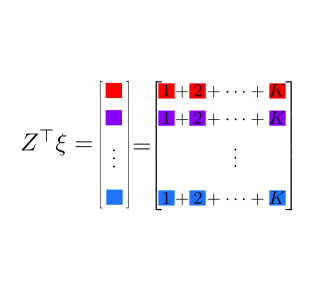
\includegraphics[scale=.3, clip, trim={1cm 8cm 1cm 8cm}]{./prebuilt_images/Ztranspose_matvec.pdf}
	\caption{Matrix-vector product for $Z^\top$ where $K$ should be big enough to avoid any error but
	also small enough to keep the power of a matrix product.}
	\label{fig:mat_trans}
\end{figure}

And for each row, the $k-th$ sub-block, $1\leq k\leq K$ is computed as follows in \Cref{fig:compute_sub_block}.
\begin{figure}[htbp]
	\centering
	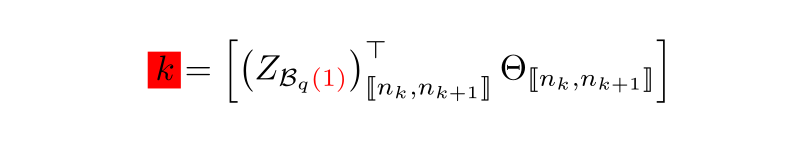
\includegraphics[scale=.2]{./prebuilt_images/prod_matvectrans_block.pdf}
	\caption{Compute the $k-th$ sub-block of the matrix-vector with the interaction matrix. This example
	is for the first main row with $p$ lines. For the $j-th$ main row, the first line uses the coefficients from $x_j\odot x_j$
	but the last line always uses those from $x_j\odot x_p$. Each sub-block $k$ is of size $n_k$ (for example the quotient of $n$ by $k$,
	$\pm 1$ to reach $n$ at the end).}
	\label{fig:compute_sub_block}
\end{figure}

%%%%%%%%%%%%%%%%%%%%%%%%%%%%%%%%%%%%%%%
%% FULL vs not FULL
%%%%%%%%%%%%%%%%%%%%%%%%%%%%%%%%%%%%%%%

\paragraph{Double interactions equivalence.} As of now, the vector $\Theta$ we considered belonged in $\bbR^{\frac{p(p+1)}{2}}$.
This implied that we removed all the feature-interactions which occured more than once in the matrix $Z$.
However, we could also consider to keep all of the interactions, meaning have $\widetilde Z\in\bbR^{n\times p^2}$ and $\widetilde\Theta\in\bbR^{p^2}$
the full versions, with a supplementary constraint on the symmetry of the coefficients in $\widetilde\Theta$.
\begin{equation}\label{eq:full}
(\cP_2) \quad \widehat{p}
	 = \min_{\substack{\beta \in \bbR^p \\ \widetilde \Theta \in \bbR^{p\times p}}}
	\frac{1}{2n}\norm{y - X\beta - \widetilde Z\widetilde \Theta}_2^2 + g^{(1)}(\beta) + g^{(2)}(\widetilde \Theta) + \iota(\widetilde \Theta_{\tau_{\widetilde q}(i,j)}=\widetilde \Theta_{\tau_{\widetilde q}(j,i)}) \enspace.
\end{equation}

where $\iota(\widetilde \Theta_{\tau_{\widetilde q}(i,j)}=\widetilde \Theta_{\tau_{\widetilde q}(j,i)}) = 0$ if the condition is verified and $+\infty$ o.w.
First, we study $y - X\beta - \widetilde Z\widetilde \Theta$, with the symmetry constraint:

\begin{align*}
	y - X\beta - \widetilde Z\widetilde \Theta
	& = y - X\beta - \sum_{(i,j)\in [p]^2} \widetilde Z_{ij} \widetilde \Theta_{ij} \\
	& = y - X\beta - 2\sum_{i\in[p]}\sum_{j>i} \widetilde Z_{\tau_q(i,j)} \widetilde \Theta_{\tau_q(i,j)} - \sum_{i\in [p]} \widetilde Z_{\tau_q(i,i)} \widetilde \Theta_{\tau_q(i,i)} \\
	& = y - X\beta - \sum_{i\in[p]}\sum_{j>i} \widetilde Z_{\tau_q(i,j)} 2\widetilde \Theta_{\tau_q(i,j)} - \sum_{i\in [p]} Z_{\tau_q(i,i)} \Theta_{\tau_q(i,i)}\enspace.
\end{align*}

Posing $\Theta_{\tau_q(i,j)} = 2 \widetilde\Theta_{\tau_q(i,j)}$ for $i\neq j$, we thus get

\begin{align*}
	\frac{1}{2n}\norm{y - X\beta - \widetilde Z\widetilde \Theta}_2^2 &= \frac{1}{2n}\norm{y - X\beta - \sum_{i\in[p]}\sum_{j>i} Z_{\tau_q(i,j)} \Theta_{\tau_q(i,j)} - \sum_{i\in [p]} Z_{\tau_q(i,i)} \Theta_{\tau_q(i,i)}}_2^2 \\
	&= \frac{1}{2n}\norm{y - X\beta - Z \Theta}_2^2 \enspace.
\end{align*}

We can execute the same decomposition on the penalties depending on $\widetilde\Theta$.
This leads to modifying $g^{(2)}$ as follows:

\begin{align*}
	g^{(2)}(\widetilde\Theta)
	&= \lambda_{\widetilde\Theta, \ell_1} \sum_{i\in [p]}\normeabs{\widetilde\Theta_{\tau_q(i,i)}} + 2\lambda_{\widetilde\Theta, \ell_1} \sum_{i>j} \normeabs{\widetilde\Theta_{\tau_q(i,j)}} +
 \frac{\lambda_{\widetilde\Theta, \ell_2}}{2} \sum_{i\in [p]}\widetilde\Theta_{\tau_q(i,i)}^2 + \lambda_{\widetilde\Theta, \ell_2}\sum_{i>j} \widetilde\Theta_{\tau_q(i,j)}^2 \\
 	& = \lambda_{\Theta, \ell_1} \sum_{i\in [p]}\normeabs{\widetilde\Theta_{\tau_q(i,i)}} + \lambda_{\Theta, \ell_1} \sum_{i>j} \normeabs{\Theta_{\tau_q(i,j)}} +
	 \frac{\lambda_{\Theta, \ell_2}}{2} \sum_{i\in [p]}\Theta_{\tau_q(i,i)}^2 + \frac{\lambda_{\Theta, \ell_2}}{2}\sum_{i>j} \left(\frac{\Theta_{\tau_q(i,j)}}{\sqrt{2}}\right)^2 \enspace,
\end{align*}

using the same variable change for non-diagonal terms. Considering as reference the problem in dimension $q=p(p+1)/2$, then we only need to mutliply instead of divide in the $\ell_2$ penalty.
So to resume, solving $(\cP)$ in dimension $q$ is equivalent to solving:


\begin{multline}\label{eq:equiv_full}
	(\widetilde\cP) \quad \widehat{p}
	 = \min_{\substack{\beta \in \bbR^p \\ \widetilde \Theta \in \bbR^{p\times p}}}
	\frac{1}{2n}\norm{y - X\beta - \widetilde Z\widetilde \Theta}_2^2 + g^{(1)}(\beta) \\
	 + \lambda_{\Theta, \ell_1}\norm{\widetilde\Theta}_1 + \frac{\lambda_{\Theta, \ell_2}}{2}\sum_{i\in[p]} \widetilde\Theta_{\tau_{\widetilde q(i,i)}}
	 + \lambda_{\Theta, \ell_2}\sum_{i\in [p]}\sum_{j>i} \widetilde \Theta_{\tau_{\widetilde q(i,j)}}^2 + \iota(\widetilde \Theta_{\tau_{\widetilde q}(i,j)}=\widetilde \Theta_{\tau_{\widetilde q}(j,i)}) \enspace.
\end{multline}

We can then compute the proximal operator for the $\widetilde\Theta$ part as before with the separability of the components \citep[p.~135]{Beck17}, which leads to:

\begin{itemize}
	\item if $i=j$:
	\[\prox_{\mu\lambda_{\Theta, \ell_1}\left(|\cdot| + \frac{\lambda_{\Theta, \ell_2}/\lambda_{\Theta, \ell_1}}{2}(\cdot)^2\right)}(t)=\frac{\sign(t)}{1+\mu\lambda_{\Theta, \ell_2}}(|t| - \mu\lambda_{\Theta, \ell_1})_+ \enspace,\]
	\item if $i\neq j$:
	\[\prox_{\mu\lambda_{\Theta, \ell_1}\left(|\cdot| + 2\frac{\lambda_{\Theta, \ell_2}}{\lambda_{\Theta, \ell_1}}(\cdot)^2\right)}(t)=\frac{\sign(t)}{1+2\mu\lambda_{\Theta, \ell_2}}(|t| - \mu\lambda_{\Theta, \ell_1})_+ \enspace.\]

\end{itemize}

%%%%%%%%%%%%%%%%%%%%%%%%%%%%%%%%%%%%%%%
%% CBPG
%%%%%%%%%%%%%%%%%%%%%%%%%%%%%%%%%%%%%%%

\paragraph{Cyclic Block Proximal Gradient (CBPG).} With the current proximal gradient descent, we update all of the coordinates of
the two vectors $\beta$ and $\Theta$ together. If we'd use a coordinate descent \citep{Bascou_Lebre_Salmon20}, in each epoch we need to update each coordinate, one at a
time, for the two vectors. To use a compromise between them, we can exploit the block structure of the interaction matrix.
Thus, for the vector $\Theta$, we can make updates by blocks \citep{massias2019sparse,Beck17}. By doing so, we need the expression of the derivative involved for
each block and the associated Lipschitz constants.
Both can be retrieved using the same method as before, so we get:

\begin{itemize}
	\item $\frac{\partial}{\partial \Theta_{\branch{q}{i}}}f(\beta, \Theta) = \frac{1}{n} Z_{\branch{q}{i}}^\top (X\beta + Z\Theta - y)$,
	\item $\norm{\frac{\partial}{\partial \Theta_{\branch{q}{i}}}f(\beta, \Theta_1) - \frac{\partial}{\partial \Theta_{\branch{q}{i}}}f(\beta, \Theta_2)}_2
	\leq \frac{1}{n}\norm{Z_{\branch{q}{i}}^\top Z}_2 \norm{\Theta_1 - \Theta_2}_2$.
\end{itemize}

Denoting $L_i=\frac{1}{n}\norm{Z_{\branch{q}{i}}^\top Z}_2$ the Lipschitz constant associated to the update of the $i-th$ block, we can define how to do an epoch.

\begin{algorithm}[H]
\label{algo:Algorithm_blockupdate}
\caption{Cyclic block proximal gradient for one epoch at iteration $k\geq 1$}
\SetKwInOut{Input}{Input~}
\SetKwInOut{Output}{Output~}
\Input{$X\in \bbR^{n\times p}$, $y\in\bbR^{n}$}

$\beta^{k+1} =  \prox_{\frac{1}{L_X}g^{(1)}}\left(\beta^k - \frac{1}{L_X}\frac{\partial}{\partial \beta}f(\beta^k, \Theta^k)\right)$,

\FOR{$i=1,\dots,p$}{
	$ \Theta^{k+1}_{\branch{q}{i}}= \prox_{\frac{1}{L_i}g^{(2)}}\left(\Theta^k_{\branch{q}{i}} - \frac{1}{L_i}\frac{\partial}{\partial \Theta_{\branch{q}{i}}}f(\beta^{k+1}, \Theta^k)\right)$
}

\Output{$\beta, \Theta$}
\end{algorithm}

%%%%%%%%%%%%%%%%%%%%%%%%%%%%%%%%%%%%%%%%%%%%%%%%%%%%%
%% Need to at least talk about the power method once
%%%%%%%%%%%%%%%%%%%%%%%%%%%%%%%%%%%%%%%%%%%%%%%%%%%%%

\paragraph{Step-size for the interaction matrix.} The last element needed for all the methods in the computation of the step for the interaction
matrix. Essentially, we need to be able to compute or have a good upper bound for $\norm{Z^\top Z}_2$ or for a fixed $i\leq p$, $\norm{Z_{\branch{q}{i}}^\top Z}_2$.
To do so, several methods are avaible. Below we present the one used and compare the bounds to made a choice between two results available.

\medskip

First in the PGD, for $\norm{Z^\top Z}_2$, we can simply use the power method \citep{golub2000eigenvalue} to get the exact value.
However, using this method on CBPG with $p$ blocks becomes very costly (especially considering that $Z_{\branch{q}{i}}^\top Z$ is not squared so we have to apply the power
method on $Z^\top Z_{\branch{q}{i}}Z_{\branch{q}{i}}^\top Z$). An alternative is to consider not the exact value but an upper bound with reasonable computation cost.
Such a bound could be computed from the consistency of the operator norm, \ie $\norm{Z_{\branch{q}{i}}^\top Z}_2 \leq \norm{Z_{\branch{q}{i}}}_2 \norm{Z}_2$.

\begin{figure}[t]
	\begin{subfigure}{.45\textwidth}
		\centering
		\includegraphics[scale = 0.44]{./prebuilt_images/lipschitz_values_sklearndata.pdf}
		\caption{$p=150$ and $n=100$ on simulated dataset from the \texttt{make\_regression} function of \texttt{Scikit-learn}.}
	\end{subfigure}
	\begin{subfigure}{.45\textwidth}
		\centering
		\includegraphics[scale = 0.43]{./prebuilt_images/lipschitz_values_genomdata.pdf}
		\caption{$p=531$ and $n=19393$ on a genomic dataset (see \nameref{par:genom}).}
	\end{subfigure}
	\caption{Comparison of upper bounds on two simulated datasets for $\norm{Z_{\branch{q}{i}}^\top Z}_2$.}
	\label{fig:lip_values}
\end{figure}

As we see in \Cref{fig:lip_values}, the majoration produced can lead to quite far results, which could lead to very slow convergence during computation.
But, contrary to the power method, it is actually very fast to compute using the Cauchy-Schwarz inequality.
For the next part, recall that $Z\in\bbR^{n\times q}$ and $Z_{\branch{q}{i}}\in\bbR^{n\times p_i}$.
For any matrix $K=(k_{ij})_{i,j}\in\bbR^{n_1\times n_2}$, we have \citep[p.~27]{vandebril07}:
\begin{align}\label{eq:max_bound}
\norm{K}_2 \leq \sqrt{n_1n_2}\max_{i,j} |k_{ij}| \enspace.
\end{align}

Applying \eqref{eq:max_bound} to $K=Z_{\branch{q}{i}}^\top Z$, for each $1\leq i\leq p$, we could compute $K$ by blocks and get the maximum component each time.
But we can even go faster using Cauchy-Schwarz inequality. Indeed, we want to perform our algorithms on the standardized matrix $Z$. So for any $i$,
$K$ is only a subset of the Gram matrix made from $Z$. Thus for $l\in[p_i]$ and $m\in[q]$:

\[|k_{lm}| = |\left\langle Z_{\tau_q(i,l)}\, |\,  z_m\right\rangle | \leq \norm{Z_{\tau_q(i,l)}}_2 \norm{z_m}_2 \leq n\enspace,\]

because with a standardized matrix $Z$, $\norm{z_m}_2^2 = n \Var(z_m)=n$.
And this bound is reached when $\tau_q(i, l)=m$, so for each block $Z_{\branch{q}{i}}$, we have:

\[\norm{Z_{\branch{q}{i}}^\top Z}_2 \leq n\sqrt{q\times p_i} \enspace.\]

The goal now is to improve the time consumption of the estimation of the largest singular value without losing too much in precision.
We can indeed do better (see \Cref{fig:lanczos}) than the power method using the Lanczos algorithm \Citep{lanczos1952solution} without sacrifying the precision.
The core idea is quite simple. Where the power method iterates through the Krylov space and only keep the last iterate to generate a new direction, Lanczos uses more deeply the Krylov space exploration made in all the past iterations.
Note that this is not a method to directly compute the largest eigenvalue, but more generally it is a way to approximate all of the eigenvalues of a (potentially very large) hermitian matrix by considering a smaller matrix $T$.
The matrix $T$ generated is in fact the orhogonal projection of the original matrix onto a Krylov subspace.
We have the relation \[T = V^* H V\enspace,\]
thus if $x$ is an eigenvector of a matrix $H$, then $Vx$ is an eigenvector of $T$ for the same eigenvalue, where $V$ and $T$ are constructed by Lanczos method.
\medskip

\begin{algorithm}[H]
	\label{algo:Lanczos}
	\caption{Lanczos algorithm on an hermitian matrix H}
	\SetKwInOut{Input}{Input~}
	\SetKwInOut{Output}{Output~}
	\Input{$H\in \bbR^{n\times n}$, $m$ dimension of the Krylov subspace visited}

	$v_1$ random unit vector

	\FOR{$j=1,\dots,m-1$}{
		$ w_{j+1} = Hv_j$ \hspace{3cm} // visit a new direction \\
		$t_{k,j} = \langle v_k, w_{j+1} \rangle,\ k=1,\dots, j$ \\
		$w_{j+1} = w_{j+1} - \sum_{k=1}^j t_{k,j} v_k$  \hspace{.8cm} // orthogonalization\\
		$t_{j+1,j} = \|w_{j+1}\|$ \\
		$v_{j+1} = \frac{w_{j+1}}{t_{j+1, j}}$
	}

	\Output{$T$}
\end{algorithm}

Algorithm \ref{algo:Lanczos} is quite general but shows that the basis fot this method is indeed the power method, slightly modified.
In the case of $H$ hermitian, it is possible to show that $T$ is a tridiagonal matrix. Indeed $\{v_1, \dots, v_m\}$ is built to be orthogonal and:
\[\forall i < j-1,\exists \alpha_1, \dots, \alpha_k \in \bbR,\   w_{i+1} = Hv_i = \sum_{k=1}^{j-1} \alpha_k v_k\enspace. \]
Thus,

\begin{align*}
	t_{i, j} &= \langle v_i, w_{j+1}\rangle = 0,\ |i|<j-1,\\
	t_{j-1, j} &= \langle v_{j-1}, w_{j+1}\rangle = v_{j-1}^\top H v_{j} = v_{j}^\top H^\top v_{j-1} = \langle v_j, w_j\rangle = t_{j, j-1}\enspace. \\
\end{align*}

Taking $H=X^\top X$ with $X \in \bbR^{n\times p}$ simulated from a standard gaussian we compare the time and precision for the power method, Lanczos algorithm and \texttt{linalg} module of \texttt{PyTorch} to get $\|T\|_2$.
We allow $10$ iterations on the power method, and visit a subspace of dimension $10$ with Lanczos method.

\begin{figure}[!h]
	\begin{subfigure}{.45\textwidth}
		\centering
		\includegraphics[scale = 0.44]{./prebuilt_images/benchmark_powermethod_scipy_n20000p550.pdf}
		\caption{Time to produce the result}
	\end{subfigure}
	\begin{subfigure}{.45\textwidth}
		\centering
		\includegraphics[scale = 0.43]{./prebuilt_images/benchmark_powermethod_scipy_values_n20000p550.pdf}
		\caption{Values of the largest singular value obtained.}
	\end{subfigure}
	\caption{Comparison of the linalg module of \texttt{Pytorch}, the power method and Lanczos algorithms to get the largest singular value of an hermitian matrix with $n=20000$ and a varying number of features up to $550$ }
	\label{fig:lanczos}
\end{figure}

%%%%%%%%%%%%%%%%%%%%%%%%%%%%%%%%%%%%%%%
%% Stopping criterion (to move smw later)
%%%%%%%%%%%%%%%%%%%%%%%%%%%%%%%%%%%%%%%
\paragraph{Stopping criterion}

To stop our solver, we can consider to look at the distance of the current iterate to the subdifferential of the primal.
Simplifying the lines hereafter, let's consider a general Elastic-Net problem with $W\in\bbR^{n\times p}$:
\[(\mathcal{P}_{enet})\ \argmin_{w\in\bbR^n} \frac{1}{2n} \|Ww - y\|^2_2 + \lambda_1 \|w\|_1 + \frac{\lambda_2}{2}\|w\|^2_2\enspace.\]
We want to stop when $w$ is such that $d_{\|\cdot\|}(0, \partial\mathcal{P}(w))\leq \epsilon$ for $\epsilon > 0$.
This is the same as solving
\[\inf_{g\in \partial\mathcal{P}(w)} \|g\|\leq\epsilon\enspace.\]
\smallskip

First, we consider the problem coordinate-wise.
If $g\in\partial\mathcal{P}(w)$ then for $j\in [p]$,
\[g_j \in \frac{1}{n} W_j^\top (y - W w) + \lambda_1 \partial_{|\cdot|}(w_j) + \lambda_2 w_j\enspace.\]

Denoting $r=y - Ww$, we get:

\begin{align}
	\inf_{g\in\partial\mathcal{P}(w)} |g_j|
			&= d\left(\frac{1}{n} W_j^\top r + \lambda_2 w_j,  \lambda_1\partial_{|\cdot|}(g_j) \right) \\
			&= \inf_{\eta_j \in \partial_{|\cdot|}(g_j)} \frac{1}{n} \left| x_j^\top r - n \lambda_2 w_j  - n \lambda_1 \eta_j\right| \\
			&= \frac{1}{n} \left| \mathrm{ST}\left( W_j^\top r - n \lambda_2 w_j, n\lambda_1 \right) \right| \enspace.  \label{eq:stop_coord}
\end{align}

We can then stop the solver when the maximum value for $j\in[p]$ of \Cref{eq:stop_coord} is below $\epsilon$.
This strategy can be applied to our interaction problem considering that $W = [X \,|\, Z]$ and $w=[\beta, \Theta]$. Doing so we get:
\begin{align} \label{eq:stop_inter}
	\inf_{g\in\partial\mathcal{P}(w)} |g_j|
			&= \frac{1}{n} \left| \mathrm{ST}\left( W_j^\top r - n [\lambda_{\beta_, \ell_2} \mathds{1}(j \leq p) + \lambda_{\Theta_, \ell_2} \mathds{1}(j > p)] w_j, n[\lambda_{\beta_, \ell_1} \mathds{1}(j \leq p) + \lambda_{\Theta_, \ell_1} \mathds{1}(j > p)] \right) \right| \enspace.
\end{align}

\subparagraph{Equivalence LASSO KKT violation}

Because the Elastic-Net can be rewritten as a LASSO problem, \Cref{eq:stop_coord} can also be derived from the KKT violation of such a formulation.
Indeed, we have:

\begin{align*}
	\frac{1}{2n}\norm{y-Ww}_2^2 + \lambda_1 \|w\|_1 + \frac{\lambda_2}{2}\|w\|^2_2
	& = \frac{1}{2n}\norm{y-Ww}_2^2 + \lambda_1 \|w\|_1 + \sum_{j=1}^p\left(\frac{\sqrt{\lambda_2}}{2}w_j\right)^2 \\
	& = \frac{1}{2n}\left[\norm{y-Ww}_2^2 + \sum_{j=1}^p\left(\sqrt{\lambda_2 n}w_j\right)^2\right] + \lambda_1 \|w\|_1  \\
	& = \frac{1}{2n}\norm{\widetilde y - \widetilde Ww}_2^2 + \lambda_1 \|w\|_1 \enspace,
\end{align*}

with $\widetilde W=\begin{bmatrix} W \\ \sqrt{\lambda_2 n}\mathrm{Id}_{p\times p}\end{bmatrix}$ and $\widetilde y = [y \,|\, 0_p ]^\top$.
The KKT violation criterion for this problem is then to stop when:
\[\max_{j\in [p]}  \frac{1}{n} \left|\mathrm{ST}\left(\widetilde W_j^\top\widetilde r, n\lambda_1 \right)\right|\leq \epsilon\enspace.\]

When working with interactions, \Cref{pb:init} can be rewritten as a weighted LASSO objective:
\[(\cP) = \min_{\beta, \Theta}\frac{1}{2n} \|\widetilde y - \widetilde X \beta - \widetilde Z\Theta\|_2^2 + \lambda_{\beta, \ell_1} \norm{\beta}_1 + \lambda_{\Theta, \ell_1} \norm{\Theta}_1\enspace,\]
with $\widetilde y=[y\,|\, 0_p \,|\, 0_q]^\top$, $\widetilde X = \begin{bmatrix} X \\ \sqrt{\lambda_{\beta, \ell_2} n}\mathrm{Id}_{p\times p}\\ 0 \end{bmatrix}$ and $\widetilde Z = \begin{bmatrix} Z \\ 0 \\ \sqrt{\lambda_{\Theta, \ell_2} n}\mathrm{Id}_{q\times q} \end{bmatrix}$.
To recover a weighted-LASSO, we concatenate both matrices. We denote $\widetilde W = [\widetilde X \,|\, \widetilde Z]$, $\widetilde w = [\beta \,|\, \Theta]$, and $\lambda=(\lambda_{\beta, \ell_1}\mathbf{1}_p, \lambda_{\Theta, \ell_1}\mathbf{1}_q)$ we thus get:
\[(\cP) = \min_{\widetilde w}\frac{1}{2n} \| y - \widetilde W \widetilde w\|_2^2 + \sum_{j=1}^{p+q} \lambda_j |\widetilde w_j|\enspace.\]
This leads to the rewritting of \Cref{eq:stop_inter} as a LASSO problem, we can stop the solver when:
\[\max_{j\in [p+q]} \frac{1}{n} \left| \mathrm{ST}\left( \widetilde W_j^\top \widetilde r, n\lambda_j\right)\right|\leq \epsilon\enspace. \]


%%%%%%%%%%%%%%%%%%%%%%%%%%%%%%%%%%%%%%%
%% Results on datasets
%%%%%%%%%%%%%%%%%%%%%%%%%%%%%%%%%%%%%%%
\paragraph{Experimentations with datatypes, GPU and CPU.}

For our solvers, the CD method uses \texttt{Numba} with \texttt{Numpy} as backend. Other solvers use \texttt{Pytorch} with \texttt{CUDA} enabled to use GPU speed-up.
The steps are computed using the Lanczos method and after applying $\texttt{linalg}$ backend on the matrix $T$, with a subspace of dimension $20$.
The computation of the criterion value and the objective are made through a callback inside the solver. This lets us get the informations at
different iterates without having to run the solver again from scratch. The time to compute these informations is removed from the benchmark.
Simulated dataset are made from Gaussian variables. When the signal to noise ratio is fixed, it is computed from:
\[\mathrm{SNR} = \frac{\var(Y)}{\var(\varepsilon)}, \text{ with }\varepsilon \sim \mathcal{N}(0, \sigma^2\mathrm{Id})\enspace.\]

\medskip

One can always wonder if there is an interest about using a more complex architecture such as GPUs in this framework. Here, we simulated a dataset
with $n=20000$, $p=500$ of type doubles. We stop the solvers when they break through $\epsilon=10^{-5}$ precision or when the curve flattens and look at the difference between using CUDA or
stay purely on CPU for the PGD and CBPG methods.
It is clear from \Cref{fig:cuda_nocuda} that, when working with these solvers, using GPU acceleration lead to results avaiable in much fewer time.
It is well known and documented by the libraries \citep{torch} that GPUs should be used with \texttt{float32} precision for better performance.
However, our methods can accumulate some rounding errors that are amplified. \Cref{fig:float} shows the time-precision trade-off we need to choose from in our computation.
As a side-note, it should be noted that to this day, in \texttt{Numba}, when accessing one coefficient from a \texttt{Numpy} array, even if the original array is in $35$-precision, the accessed values is casted to $64$-precision internally because of \texttt{CPython}.


\begin{figure}[!h]
	\begin{subfigure}{.45\textwidth}
		\centering
		\includegraphics[scale=.4]{./prebuilt_images/cuda_vs_nocuda_simulated_n20000p500.pdf}
		\caption{KKT violation criterion with CUDA vs no CUDA for PGD and CBPG with simulated data of $20000$ samples and $500$ features.}
		\label{fig:cuda_nocuda}
	\end{subfigure}
	\begin{subfigure}{.45\textwidth}
		\centering
		\includegraphics[scale=.4]{./prebuilt_images/float_comparison_n25000p400.pdf}
		\caption{Effect of 32 or 64-bits precision on CBPG and PGD methods in
		a simulated dataset with $n=25000$ and $p=400$.}
		\label{fig:float}
	\end{subfigure}
	\caption{Float64 lead to better precision but at a higher cost in time and using CUDA acceleration with Float32 result in less time consuming solvers.}
	\label{fig:floating_point}
\end{figure}

\paragraph{Experimentations with simulated datasets.}

For now, we chose to use a simulated regression dataset with $p=500$ features and $n=20000$. We also fixed the signal to noise ratio to $10$.
We denote the regularizations $\lambda_{\max}$ as the maximum between $\lambda_{\Theta,\ell_1}=\lambda_{\beta, \ell_1}\simeq 843.228$ and $\lambda_{\Theta,\ell_2}=\lambda_{\beta, \ell_2}\simeq 128.588$.
\begin{figure}[ht!]
	\begin{subfigure}{.45\textwidth}
		\centering
		\includegraphics[scale = 0.38]{prebuilt_images/simulated_n20000p500_kkt_snr10.pdf}
		\caption{Regularizations are set to $\frac{\lambda_{\max}}{10}$.}
		\label{fig:simu_ccl}
	\end{subfigure}
	\begin{subfigure}{.45\textwidth}
		\centering
		\includegraphics[scale = 0.38]{prebuilt_images/simulated_n20000p500_kkt_snr10_over100.pdf}
		\caption{Regularizations are set to $\frac{\lambda_{\max}}{100}$.}
		\label{fig:simu_ccl_over100}
	\end{subfigure}
	\caption{KKT criterion curves on the simulated regression dataset with $n=20000$ and $p=500$, $q=\frac{p(p+1)}{2}$.
	Maximum number of epochs is set to $100$. Float types are $32$-bytes.
	}
\end{figure}

As we see in \Cref{fig:simu_ccl}, Coordinate Descent is still faster for very sparse solutions. But descreasing the regularisations to $\frac{\lambda_{\max}}{100}$ with the same signal to noise
ratio leads to methods on GPU being equal or faster than coordinate descent. These simulations were made with a sparsity in $\beta$ and $\Theta$ of $25\%$ (meaning $25\%$ of the coefficients were active).
We wondered how sparser solutions could affect the solvers.

\begin{figure}[ht]
	\centering
	\includegraphics[scale=.4]{prebuilt_images/simulated_n20000p500_kkt_snr10_over100_sp.pdf}
	\caption{KKT criterion curves on the simulated regression dataset with $n=20000$, $p=500$, $\mathrm{SNR}=10$, sparsity levels of $1\%$ in $\beta$ and $\Theta$, regularizations to $\frac{\lambda_{\max}}{100}$, Float-$32$ types and $100$ epochs allowed.}
	\label{fig:sparsity_solvers}
\end{figure}

With very sparse solutions, \Cref{fig:sparsity_solvers} shows that coordinate descent methods have more advantages and lead over PGD. Here however CBPG methods are still better.
We can wonder if deviding regularizations by such factors are realistic (especially since we set the sparsity level to $1\%$ in our simulated dataset). To look at that we traced the surface plot
of the sparsity level obtained in the vector $\Theta$ (very large) against the regularizations. As we can see in \Cref{fig:sp_surf} if the $\ell_1$ regularization is high, we recover the good level of sparsity.
But it is also in this situation that the coordinate descent is faster.

\begin{figure}[ht]
	\centering
	\includegraphics[scale=.4]{prebuilt_images/theta_surface_sparsity.pdf}
	\caption{Sparsity obtained in $\Theta$ with $n=20000$, $p=500$, $\mathrm{SNR}=10$, sparsity level simulated of $1\%$ in $\beta$ and $\Theta$, Float-$32$ types and $100$ epochs allowed.}
	\label{fig:sp_surf}
\end{figure}

We see that our GPU-accelerated methods are faster with smaller regularizations and might seem not very useful, albeit it is not often that we know per advance the right regularization to choose from.
In most cases, a set (or grid) of parameters is given to our method, we look at the obtained Mean Squared Error (or any other criterion) and select the regularization that lead to the best performance.
The key hypothesis is that we might not have any prior idea about the location of the best parameters. In this situation, one can choose a grid search of $\frac{\lambda_{\max}}{\ell_1\ \text{factor}}$ for the $\ell_1$ regularization. Let's use $\lambda_{\ell_2}=\frac{\lambda_{\max}}{10}$ and see for varying $\ell_1$ regularizations the time spent and the MSE obtained.
Also, doing so we don't need to compute each time the Lipschitz constants of all the blocks in the Cyblic Block method, they are computed for one run and the next ones can reuse them.

\begin{figure}[ht!]
	\begin{subfigure}{.45\textwidth}
		\centering
		\includegraphics[scale = 0.43]{prebuilt_images/simulated_n20000p500_snr=10_TIME.pdf}
		\caption{Time consumption with varying $\ell_1$ penalty.}
		\label{fig:time_search}
	\end{subfigure}
	\begin{subfigure}{.45\textwidth}
		\centering
		\includegraphics[scale = 0.43]{prebuilt_images/simulated_n20000p500_snr=10_MSE.pdf}
		\caption{MSE with varying $\ell_1$ penalty.}
		\label{fig:mse_search}
	\end{subfigure}
	\caption{On simulated regression dataset with $n=20000$ and $p=500$, $q=\frac{p(p+1)}{2}$.
	Maximum number of epochs is set to $500$ but solvers stop if the criterion is achieved. Float types are $32$-bytes. KKT criterion is set to $10^{-3}$. SNR is set to $10$. Sparsity levels are at $1\%$}
\end{figure}

As we see in \Cref{fig:mse_search} all our errors are close. And with \Cref{fig:time_search} we see the three situations we encountered before. Around a division of $\lambda_{\max}$ by $10$ and before, CD is faster.
After that CD is better than PGD-type methods but not CBPGs. And then it needs to search even longer. Note that in this experiment, only PGD methods did not reach the $\epsilon=10^{-3}$ precision in the $500$ epochs allowed for the last regularizations (hence the flattening curve meaning we only see the time it takes to make the maximum number of epochs).
And although it appears the MSE curve is decreasing, actually the MSE for the last regularization is higher than the one for the penultimate's near $400$.
And because we are in a fully simulated problem, with values in $\beta$ between $-1000$ and $1000$ and values for $\Theta$ bewteen $-100$ and $100$, we can check the MSE between the obtained iterates and the true coefficients in \Cref{fig:mse_coeffs}:

\begin{figure}[ht!]
	\begin{subfigure}{.45\textwidth}
		\centering
		\includegraphics[scale = 0.43]{prebuilt_images/simu_total/simulated_n20000p500_snr=10_difftheta_2605.pdf}
		\caption{$\frac{1}{q}\|\widehat \Theta - \Theta\|^2_2$.}
		\label{fig:mse_theta}
	\end{subfigure}
	\begin{subfigure}{.45\textwidth}
		\centering
		\includegraphics[scale = 0.43]{prebuilt_images/simu_total/simulated_n20000p500_snr=10_diffbeta_2605.pdf}
		\caption{$\frac{1}{p}\|\widehat \beta - \beta\|^2_2$.}
		\label{fig:mse_beta}
	\end{subfigure}
	\caption{MSE in simulated regression dataset with $n=20000$ and $p=500$, $q=\frac{p(p+1)}{2}$.
	Maximum number of epochs is set to $500$ but solvers stop if the criterion is achieved. Float types are $32$-bytes. KKT criterion is set to $10^{-3}$. SNR is set to $10$. Sparsity levels are at $1\%$}
	\label{fig:mse_coeffs}
\end{figure}


\paragraph{Experimentations with a genomic dataset} \label{par:genom}

To test this method and see the time consumption, we used a genomic dataset \citep{Bessiere_Taha_Petitprez_Vandel_Marin_Brehelin_Lebre_Lecellier}
with a sample size of $n=19393$ and $p=531$ features.
The total number of interactions (squared included) is thus $q=\frac{1}{2}p(p+1)=141246$, so the matrix $Z$ of size $n\times q$
can not be stored on most GPUs. As response, we keep the first column amongst all the responses available.
We also compared the results with a \emph{random CBPG} wich consists on applying $p$ updates of blocks of the matrix $Z$ but with a sampler to know which block should be updated.
This method is described in \Citep{nesterov2012efficiency} and is implemented with the $O(\log n)$ sampler did not lead to better results.
We let the solvers run at most $100$ epochs. We are in float-$32$ precision, looking at the KKT violation criterion.

\begin{figure}[!h]
	\begin{subfigure}{.45\textwidth}
	\centering
	\includegraphics[scale=.43]{prebuilt_images/simulated_n19393p531_snrgenom_MSE_rd.pdf}
	\caption{MSE on test set.}
	\end{subfigure}
	\begin{subfigure}{.45\textwidth}
	\includegraphics[scale=.43]{prebuilt_images/simulated_n19393p531_snrgenom_TIME_rd.pdf}
	\caption{Time for solvers to end.}
	\end{subfigure}
	\caption{Benchmark of CBPG and CD on the genomic dataset. The data has $n=19393$ samples of $p=531$ features. Train set is $75\%$ of the dataset.
    Maximum number of epochs allowed is $100$.}
	\label{fig:bench_genom}
\end{figure}


%%%%%%%%%%%%%%%%%%%%%%%%%%%%%%%%%%%%%%%
%% Conclusion
%%%%%%%%%%%%%%%%%%%%%%%%%%%%%%%%%%%%%%%
\section*{Conclusion}

We worked on a model with interactions that can't be stored on devices and used gradient descent algorithms as solvers.
We also considered the problem with $p^2$ interactions leading to a slightly-modified ElasticNet algorithm when looking for
the equivalence with the smaller problem. Working with GPU accelerated gradient descent method can lead to similar speeds and results
coordinate descent methods. To see that, we worked with the KKT violation criterion which was written for the interaction model.

%%%%%%%%%%%%%%%%%%%%%%%%%%%%%%%%%%%%%%%
%% Biblio
%%%%%%%%%%%%%%%%%%%%%%%%%%%%%%%%%%%%%%%
\newpage
\bibliography{../references.bib}

\end{document}
